%% bare_conf.tex
%% V1.4b
%% 2015/08/26
%% by Michael Shell
%% See:
%% http://www.michaelshell.org/
%% for current contact information.
%%
%% This is a skeleton file demonstrating the use of IEEEtran.cls
%% (requires IEEEtran.cls version 1.8b or later) with an IEEE
%% conference paper.
%%
%% Support sites:
%% http://www.michaelshell.org/tex/ieeetran/
%% http://www.ctan.org/pkg/ieeetran
%% and
%% http://www.ieee.org/

%%*************************************************************************
%% Legal Notice:
%% This code is offered as-is without any warranty either expressed or
%% implied; without even the implied warranty of MERCHANTABILITY or
%% FITNESS FOR A PARTICULAR PURPOSE! 
%% User assumes all risk.
%% In no event shall the IEEE or any contributor to this code be liable for
%% any damages or losses, including, but not limited to, incidental,
%% consequential, or any other damages, resulting from the use or misuse
%% of any information contained here.
%%
%% All comments are the opinions of their respective authors and are not
%% necessarily endorsed by the IEEE.
%%
%% This work is distributed under the LaTeX Project Public License (LPPL)
%% ( http://www.latex-project.org/ ) version 1.3, and may be freely used,
%% distributed and modified. A copy of the LPPL, version 1.3, is included
%% in the base LaTeX documentation of all distributions of LaTeX released
%% 2003/12/01 or later.
%% Retain all contribution notices and credits.
%% ** Modified files should be clearly indicated as such, including  **
%% ** renaming them and changing author support contact information. **
%%*************************************************************************


% *** Authors should verify (and, if needed, correct) their LaTeX system  ***
% *** with the testflow diagnostic prior to trusting their LaTeX platform ***
% *** with production work. The IEEE's font choices and paper sizes can   ***
% *** trigger bugs that do not appear when using other class files.       ***                          ***
% The testflow support page is at:
% http://www.michaelshell.org/tex/testflow/



%\documentclass[conference]{IEEEtran}
\documentclass[onecolumn,draftcls]{IEEEtran}
% Some Computer Society conferences also require the compsoc mode option,
% but others use the standard conference format.
%
% If IEEEtran.cls has not been installed into the LaTeX system files,
% manually specify the path to it like:
% \documentclass[conference]{../sty/IEEEtran}





% Some very useful LaTeX packages include:
% (uncomment the ones you want to load)


% *** MISC UTILITY PACKAGES ***
%
%\usepackage{ifpdf}
% Heiko Oberdiek's ifpdf.sty is very useful if you need conditional
% compilation based on whether the output is pdf or dvi.
% usage:
% \ifpdf
%   % pdf code
% \else
%   % dvi code
% \fi
% The latest version of ifpdf.sty can be obtained from:
% http://www.ctan.org/pkg/ifpdf
% Also, note that IEEEtran.cls V1.7 and later provides a builtin
% \ifCLASSINFOpdf conditional that works the same way.
% When switching from latex to pdflatex and vice-versa, the compiler may
% have to be run twice to clear warning/error messages.






% *** CITATION PACKAGES ***
%
\usepackage{cite}
% cite.sty was written by Donald Arseneau
% V1.6 and later of IEEEtran pre-defines the format of the cite.sty package
% \cite{} output to follow that of the IEEE. Loading the cite package will
% result in citation numbers being automatically sorted and properly
% "compressed/ranged". e.g., [1], [9], [2], [7], [5], [6] without using
% cite.sty will become [1], [2], [5]--[7], [9] using cite.sty. cite.sty's
% \cite will automatically add leading space, if needed. Use cite.sty's
% noadjust option (cite.sty V3.8 and later) if you want to turn this off
% such as if a citation ever needs to be enclosed in parenthesis.
% cite.sty is already installed on most LaTeX systems. Be sure and use
% version 5.0 (2009-03-20) and later if using hyperref.sty.
% The latest version can be obtained at:
% http://www.ctan.org/pkg/cite
% The documentation is contained in the cite.sty file itself.






% *** GRAPHICS RELATED PACKAGES ***
%
\ifCLASSINFOpdf
	\usepackage[pdftex]{graphicx}
  % declare the path(s) where your graphic files are
    \graphicspath{{Figures/}}
  % and their extensions so you won't have to specify these with
  % every instance of \includegraphics
    \DeclareGraphicsExtensions{.pdf,.jpeg,.png}
\else
  % or other class option (dvipsone, dvipdf, if not using dvips). graphicx
  % will default to the driver specified in the system graphics.cfg if no
  % driver is specified.
  % \usepackage[dvips]{graphicx}
  % declare the path(s) where your graphic files are
  % \graphicspath{{../eps/}}
  % and their extensions so you won't have to specify these with
  % every instance of \includegraphics
  % \DeclareGraphicsExtensions{.eps}
\fi
% graphicx was written by David Carlisle and Sebastian Rahtz. It is
% required if you want graphics, photos, etc. graphicx.sty is already
% installed on most LaTeX systems. The latest version and documentation
% can be obtained at: 
% http://www.ctan.org/pkg/graphicx
% Another good source of documentation is "Using Imported Graphics in
% LaTeX2e" by Keith Reckdahl which can be found at:
% http://www.ctan.org/pkg/epslatex
%
% latex, and pdflatex in dvi mode, support graphics in encapsulated
% postscript (.eps) format. pdflatex in pdf mode supports graphics
% in .pdf, .jpeg, .png and .mps (metapost) formats. Users should ensure
% that all non-photo figures use a vector format (.eps, .pdf, .mps) and
% not a bitmapped formats (.jpeg, .png). The IEEE frowns on bitmapped formats
% which can result in "jaggedy"/blurry rendering of lines and letters as
% well as large increases in file sizes.
%
% You can find documentation about the pdfTeX application at:
% http://www.tug.org/applications/pdftex





% *** MATH PACKAGES ***
%
\usepackage{amsmath}
% A popular package from the American Mathematical Society that provides
% many useful and powerful commands for dealing with mathematics.
%
% Note that the amsmath package sets \interdisplaylinepenalty to 10000
% thus preventing page breaks from occurring within multiline equations. Use:
%\interdisplaylinepenalty=2500
% after loading amsmath to restore such page breaks as IEEEtran.cls normally
% does. amsmath.sty is already installed on most LaTeX systems. The latest
% version and documentation can be obtained at:
% http://www.ctan.org/pkg/amsmath





% *** SPECIALIZED LIST PACKAGES ***
%
%\usepackage{algorithmic}
% algorithmic.sty was written by Peter Williams and Rogerio Brito.
% This package provides an algorithmic environment fo describing algorithms.
% You can use the algorithmic environment in-text or within a figure
% environment to provide for a floating algorithm. Do NOT use the algorithm
% floating environment provided by algorithm.sty (by the same authors) or
% algorithm2e.sty (by Christophe Fiorio) as the IEEE does not use dedicated
% algorithm float types and packages that provide these will not provide
% correct IEEE style captions. The latest version and documentation of
% algorithmic.sty can be obtained at:
% http://www.ctan.org/pkg/algorithms
% Also of interest may be the (relatively newer and more customizable)
% algorithmicx.sty package by Szasz Janos:
% http://www.ctan.org/pkg/algorithmicx




% *** ALIGNMENT PACKAGES ***
%
%\usepackage{array}
% Frank Mittelbach's and David Carlisle's array.sty patches and improves
% the standard LaTeX2e array and tabular environments to provide better
% appearance and additional user controls. As the default LaTeX2e table
% generation code is lacking to the point of almost being broken with
% respect to the quality of the end results, all users are strongly
% advised to use an enhanced (at the very least that provided by array.sty)
% set of table tools. array.sty is already installed on most systems. The
% latest version and documentation can be obtained at:
% http://www.ctan.org/pkg/array


% IEEEtran contains the IEEEeqnarray family of commands that can be used to
% generate multiline equations as well as matrices, tables, etc., of high
% quality.




% *** SUBFIGURE PACKAGES ***
%\ifCLASSOPTIONcompsoc
%  \usepackage[caption=false,font=normalsize,labelfont=sf,textfont=sf]{subfig}
%\else
%  \usepackage[caption=false,font=footnotesize]{subfig}
%\fi
% subfig.sty, written by Steven Douglas Cochran, is the modern replacement
% for subfigure.sty, the latter of which is no longer maintained and is
% incompatible with some LaTeX packages including fixltx2e. However,
% subfig.sty requires and automatically loads Axel Sommerfeldt's caption.sty
% which will override IEEEtran.cls' handling of captions and this will result
% in non-IEEE style figure/table captions. To prevent this problem, be sure
% and invoke subfig.sty's "caption=false" package option (available since
% subfig.sty version 1.3, 2005/06/28) as this is will preserve IEEEtran.cls
% handling of captions.
% Note that the Computer Society format requires a larger sans serif font
% than the serif footnote size font used in traditional IEEE formatting
% and thus the need to invoke different subfig.sty package options depending
% on whether compsoc mode has been enabled.
%
% The latest version and documentation of subfig.sty can be obtained at:
% http://www.ctan.org/pkg/subfig




% *** FLOAT PACKAGES ***
%
%\usepackage{fixltx2e}
% fixltx2e, the successor to the earlier fix2col.sty, was written by
% Frank Mittelbach and David Carlisle. This package corrects a few problems
% in the LaTeX2e kernel, the most notable of which is that in current
% LaTeX2e releases, the ordering of single and double column floats is not
% guaranteed to be preserved. Thus, an unpatched LaTeX2e can allow a
% single column figure to be placed prior to an earlier double column
% figure.
% Be aware that LaTeX2e kernels dated 2015 and later have fixltx2e.sty's
% corrections already built into the system in which case a warning will
% be issued if an attempt is made to load fixltx2e.sty as it is no longer
% needed.
% The latest version and documentation can be found at:
% http://www.ctan.org/pkg/fixltx2e


%\usepackage{stfloats}
% stfloats.sty was written by Sigitas Tolusis. This package gives LaTeX2e
% the ability to do double column floats at the bottom of the page as well
% as the top. (e.g., "\begin{figure*}[!b]" is not normally possible in
% LaTeX2e). It also provides a command:
%\fnbelowfloat
% to enable the placement of footnotes below bottom floats (the standard
% LaTeX2e kernel puts them above bottom floats). This is an invasive package
% which rewrites many portions of the LaTeX2e float routines. It may not work
% with other packages that modify the LaTeX2e float routines. The latest
% version and documentation can be obtained at:
% http://www.ctan.org/pkg/stfloats
% Do not use the stfloats baselinefloat ability as the IEEE does not allow
% \baselineskip to stretch. Authors submitting work to the IEEE should note
% that the IEEE rarely uses double column equations and that authors should try
% to avoid such use. Do not be tempted to use the cuted.sty or midfloat.sty
% packages (also by Sigitas Tolusis) as the IEEE does not format its papers in
% such ways.
% Do not attempt to use stfloats with fixltx2e as they are incompatible.
% Instead, use Morten Hogholm'a dblfloatfix which combines the features
% of both fixltx2e and stfloats:
%
% \usepackage{dblfloatfix}
% The latest version can be found at:
% http://www.ctan.org/pkg/dblfloatfix




% *** PDF, URL AND HYPERLINK PACKAGES ***
%
%\usepackage{url}
% url.sty was written by Donald Arseneau. It provides better support for
% handling and breaking URLs. url.sty is already installed on most LaTeX
% systems. The latest version and documentation can be obtained at:
% http://www.ctan.org/pkg/url
% Basically, \url{my_url_here}.




% *** Do not adjust lengths that control margins, column widths, etc. ***
% *** Do not use packages that alter fonts (such as pslatex).         ***
% There should be no need to do such things with IEEEtran.cls V1.6 and later.
% (Unless specifically asked to do so by the journal or conference you plan
% to submit to, of course. )
\usepackage{unicode-math}
\usepackage{color}
\usepackage{tcolorbox}
\usepackage{subcaption}


% correct bad hyphenation here
\hyphenation{net-works}


\begin{document}
%
% paper title
% Titles are generally capitalized except for words such as a, an, and, as,
% at, but, by, for, in, nor, of, on, or, the, to and up, which are usually
% not capitalized unless they are the first or last word of the title.
% Linebreaks \\ can be used within to get better formatting as desired.
% Do not put math or special symbols in the title.
%\title{Genetic Algorithm-based Resource Allocation for Virtualized Wireless Networks}
%\title{A Genetic Algorithm Approach for Approximating Resource Allocation in Virtualized Wireless Networks with Log-Normal Distributed Traffic Demand}
\title{Joint Base Station Selection and Adaptive Slicing in Virtualized Wireless Networks with Log-Normal Distributed Traffic Demand}


% author names and affiliations
% use a multiple column layout for up to three different
% affiliations
\author{
\IEEEauthorblockN{Kory Teague, Mohammad J. Abdel-Rahman, and Allen B. MacKenzie\\}
\IEEEauthorblockA{Department of Electrical and Computer Engineering, Virginia Tech, USA \\
\{koryt, mo7ammad, mackenab\}@vt.edu
}}

\iffalse
\author{\IEEEauthorblockN{Kory Teague}
\IEEEauthorblockA{School of Electrical and\\Computer Engineering\\
Virginia Tech\\
Blacksburg, VA\\
Email: koryt@vt.edu}
\and
\\
\IEEEauthorblockN{Mohammad Abdel-Rahman}
\IEEEauthorblockA{School of Electrical and\\Computer Engineering\\
Virginia Tech\\
Blacksburg, VA\\
Email: mo7ammad@vt.edu}
\and
\\
\IEEEauthorblockN{Allen MacKenzie}
\IEEEauthorblockA{School of Electrical and\\Computer Engineering\\
Virginia Tech\\
Blacksburg, VA\\
Email: mackenab@vt.edu}}
\fi

% conference papers do not typically use \thanks and this command
% is locked out in conference mode. If really needed, such as for
% the acknowledgment of grants, issue a \IEEEoverridecommandlockouts
% after \documentclass

% for over three affiliations, or if they all won't fit within the width
% of the page, use this alternative format:
% 
%\author{\IEEEauthorblockN{Michael Shell\IEEEauthorrefmark{1},
%Homer Simpson\IEEEauthorrefmark{2},
%James Kirk\IEEEauthorrefmark{3}, 
%Montgomery Scott\IEEEauthorrefmark{3} and
%Eldon Tyrell\IEEEauthorrefmark{4}}
%\IEEEauthorblockA{\IEEEauthorrefmark{1}School of Electrical and Computer Engineering\\
%Georgia Institute of Technology,
%Atlanta, Georgia 30332--0250\\ Email: see http://www.michaelshell.org/contact.html}
%\IEEEauthorblockA{\IEEEauthorrefmark{2}Twentieth Century Fox, Springfield, USA\\
%Email: homer@thesimpsons.com}
%\IEEEauthorblockA{\IEEEauthorrefmark{3}Starfleet Academy, San Francisco, California 96678-2391\\
%Telephone: (800) 555--1212, Fax: (888) 555--1212}
%\IEEEauthorblockA{\IEEEauthorrefmark{4}Tyrell Inc., 123 Replicant Street, Los Angeles, California 90210--4321}}




% use for special paper notices
%\IEEEspecialpapernotice{(Invited Paper)}




% make the title area
\maketitle

% As a general rule, do not put math, special symbols or citations
% in the abstract
\begin{abstract}
\textcolor{blue}{\textit{The abstract goes here once written.}}
\end{abstract}

% no keywords




% For peer review papers, you can put extra information on the cover
% page as needed:
% \ifCLASSOPTIONpeerreview
% \begin{center} \bfseries EDICS Category: 3-BBND \end{center}
% \fi
%
% For peerreview papers, this IEEEtran command inserts a page break and
% creates the second title. It will be ignored for other modes.
\IEEEpeerreviewmaketitle



\section{Introduction} \label{sec:intro}
\textcolor{blue}{\textit{Provide background and expound.}}

\iffalse
\textit{In this section we include interesting and necessary background information.  Detail virtualized wireless networks, the problem being investigated, and setup the ``story'' behind the paper.  Motivations and ``why'' in a few paragraphs.}

\textit{As it stands, the problem has been simplified such that the story may not include VWN in its implementation.  Only a single network is being created from a larger pool of resources, and no resource slicing occurs.  However, this might be utilized as a foundation for further VWN research by expanding the methods with slicing and multiple derived networks.}
\fi

The rest of this paper is organized as follows.  In Section \ref{sec:model}, we detail and define the system model assumed for our resource allocation methods.  In Section \ref{sec:approach}, we consider our resource selection and demand allocation approaches.  In Section \ref{sec:sim}, we simulate the described approaches and evaluate their performance.  Finally, in Section \ref{sec:conclusion}, we discuss our conclusions and possible future extensions.
% no \IEEEPARstart
%This demo file is intended to serve as a ``starter file''
%for IEEE conference papers produced under \LaTeX\ using
%IEEEtran.cls version 1.8b and later.
% You must have at least 2 lines in the paragraph with the drop letter
% (should never be an issue)
%I wish you the best of success.

%\hfill mds
 
%\hfill August 26, 2015

%\subsection{Subsection Heading Here}
%Subsection text here.


%\subsubsection{Subsubsection Heading Here}
%Subsubsection text here.


% An example of a floating figure using the graphicx package.
% Note that \label must occur AFTER (or within) \caption.
% For figures, \caption should occur after the \includegraphics.
% Note that IEEEtran v1.7 and later has special internal code that
% is designed to preserve the operation of \label within \caption
% even when the captionsoff option is in effect. However, because
% of issues like this, it may be the safest practice to put all your
% \label just after \caption rather than within \caption{}.
%
% Reminder: the "draftcls" or "draftclsnofoot", not "draft", class
% option should be used if it is desired that the figures are to be
% displayed while in draft mode.
%
%\begin{figure}[!t]
%\centering
%\includegraphics[width=2.5in]{myfigure}
% where an .eps filename suffix will be assumed under latex, 
% and a .pdf suffix will be assumed for pdflatex; or what has been declared
% via \DeclareGraphicsExtensions.
%\caption{Simulation results for the network.}
%\label{fig_sim}
%\end{figure}

% Note that the IEEE typically puts floats only at the top, even when this
% results in a large percentage of a column being occupied by floats.


% An example of a double column floating figure using two subfigures.
% (The subfig.sty package must be loaded for this to work.)
% The subfigure \label commands are set within each subfloat command,
% and the \label for the overall figure must come after \caption.
% \hfil is used as a separator to get equal spacing.
% Watch out that the combined width of all the subfigures on a 
% line do not exceed the text width or a line break will occur.
%
%\begin{figure*}[!t]
%\centering
%\subfloat[Case I]{\includegraphics[width=2.5in]{box}%
%\label{fig_first_case}}
%\hfil
%\subfloat[Case II]{\includegraphics[width=2.5in]{box}%
%\label{fig_second_case}}
%\caption{Simulation results for the network.}
%\label{fig_sim}
%\end{figure*}
%
% Note that often IEEE papers with subfigures do not employ subfigure
% captions (using the optional argument to \subfloat[]), but instead will
% reference/describe all of them (a), (b), etc., within the main caption.
% Be aware that for subfig.sty to generate the (a), (b), etc., subfigure
% labels, the optional argument to \subfloat must be present. If a
% subcaption is not desired, just leave its contents blank,
% e.g., \subfloat[].


% An example of a floating table. Note that, for IEEE style tables, the
% \caption command should come BEFORE the table and, given that table
% captions serve much like titles, are usually capitalized except for words
% such as a, an, and, as, at, but, by, for, in, nor, of, on, or, the, to
% and up, which are usually not capitalized unless they are the first or
% last word of the caption. Table text will default to \footnotesize as
% the IEEE normally uses this smaller font for tables.
% The \label must come after \caption as always.
%
%\begin{table}[!t]
%% increase table row spacing, adjust to taste
%\renewcommand{\arraystretch}{1.3}
% if using array.sty, it might be a good idea to tweak the value of
% \extrarowheight as needed to properly center the text within the cells
%\caption{An Example of a Table}
%\label{table_example}
%\centering
%% Some packages, such as MDW tools, offer better commands for making tables
%% than the plain LaTeX2e tabular which is used here.
%\begin{tabular}{|c||c|}
%\hline
%One & Two\\
%\hline
%Three & Four\\
%\hline
%\end{tabular}
%\end{table}


% Note that the IEEE does not put floats in the very first column
% - or typically anywhere on the first page for that matter. Also,
% in-text middle ("here") positioning is typically not used, but it
% is allowed and encouraged for Computer Society conferences (but
% not Computer Society journals). Most IEEE journals/conferences use
% top floats exclusively. 
% Note that, LaTeX2e, unlike IEEE journals/conferences, places
% footnotes above bottom floats. This can be corrected via the
% \fnbelowfloat command of the stfloats package.


\section{System Model} \label{sec:model}
We consider a geographical area of width $X$ m and length $Y$ m that contains a set $\mathcal{S} = \left\{1,\, 2,\, \ldots,\, S\right\}$ of base stations (BSs) available to the Virtual Network Builder (VNB) as provided by the Resource Providers (RPs).  The rate capacity of BS $s \in \mathcal{S}$ is denoted by $r_s$, its cost is denoted by $c_s$, and its broadcasting range is denoted by $b_s$.

% Double check citations of the following paragraph.  Read the cited papers over.  Lee has similar sentence structure for the early citations, and I need to cite to be authoratative with the citation.
%Within this area is a continuous spatial distribution indicating the overall traffic demand.  It has been shown that a log-normal distribution or a mixture of log-normal distributions can approximate traffic demand in real-world cellular networks \cite{686105}, \cite{5936263}.  It has also been shown that traffic distribution is spatially correlated \cite{5936263}, \cite{eigenplaces}.  We model this spatial traffic demand using a similar, continuous form of the SSLT (Scalable, Spatially-correlated, and Log-normally distributed Traffic) model as proposed by Lee, Zhou, and Niu \cite{6554749}.

A Service Provider (SP) seeking a Virtualized Wireless Network (VWN) from the VNB is assumed to know the distribution of traffic demand within the region the VWN would cover. \iffalse From the SPs, the VNB would then have a known continuous spatial distribution indicating the overall traffic deamnd. \fi It has been shown that a log-normal distribution or a mixture of log-normal distributions can approximate traffic demand in real-world cellular networks \cite{686105}, \cite{5936263}.  It has also been shown that traffic distribution is spatially correlated \cite{5936263}, \cite{eigenplaces}.  We model the spatial traffic demand of a single SP using a similar, continuous form of the SSLT (Scalable, Spatially-correlated, and Log-normally distributed Traffic) model as proposed by Lee, Zhou, and Niu \cite{6554749}.

To generate this spatial distribution over the area of consideration, an initial Gaussian field, $\rho^G = \rho^G\left(x,\, y\right),\, x \in \left[0,\, X\right],\, y \in \left[0,\, Y\right]$, is generated by

\begin{equation}
\rho^G\left(x,\, y\right)=\frac{1}{L}\sum_{l=1}^L \cos\left(i_lx+\phi_l\right) \; \cos\left(j_ly+\psi_l\right)
\end{equation}

% Double check following paragraph for linebreak placement.  In single column, freq/phase math blocks overflowed to the margin, necessitating \sloppy.  Consider how and where to place \linebreak as another solution.  Where is appropriate in the block?  After the tilde since it satisfies a similar purpose to an equals, which latex linebreaks on?  After the comma before l \in \mathcal{L} makes sense, but it's not enough, as the part before is too long and still overflows...
\noindent \sloppy where $\mathcal{L} \eqdef \left\{1,\, 2,\, \ldots,\, L\right\}$ is a set of the products of two cosines with angular frequencies $i_l,\, j_l\, \textasciitilde\, \mathcal{U}\left(0,\, \omega_{\max}\right),\, l \in \mathcal{L}$ and phases $\phi_l,\, \psi_l\, \textasciitilde\, \mathcal{U}\left(0,\, 2\pi\right),\, l \in \mathcal{L}$.  As $L$ increases, $\rho^G$ approaches a Gaussian random field with a spatial autocorrelation dependent on $\omega_{\max}$ according to the central limit theorem.

The approximate Gaussian distribution $\rho^G$ is then normalized to $\rho^S = \rho^S(x,\, y), x \in [0,\, X], y \in [0,\, Y]$, which has a standard normal distribution.  The final log-normal distribution, $\rho = \rho(x,\, y), x \in [0,\, X], y \in [0,\, Y]$, is determined by assigning location and scale parameters $\mu$ and $\sigma$:

\begin{equation}
\rho\left(x,\, y\right) = \exp\left(\sigma \; \rho^S\left(x,\, y\right)+\mu\right)
\end{equation}

$\rho\left(x,\, y\right)$ can be sampled over the space into individual pixels as per Lee with each pixel's value indicating the number of homogeneous demand points within the pixel \cite{6554749}.  In contrast, we allow it to provide a continuous, spatially-correlated log-normal distribution depicting the demand density over the region for the SP.

Let $\mathcal{M} \eqdef \{1,\, 2,\, \ldots,\, M\}$ be the set of the SP's demand points seeking to connect to the VWN; the value of total traffic demand at each point is denoted by $d_m$.  Further let $u_{ms} \in [0,\, 1],\, m \in \mathcal{M},\, s \in \mathcal{S}$, represent the normalized capacity (with respect to $r_s$) of BS $s$ at point $m$, i.e., the normalized maximum rate that a user can receive at point $m$ from BS $s$.  $u_{ms} = 0$ when $m$ is outside the coverage area of $s$ and $u_{ms} = 1$ when $m$ is within a small distance of $s$.  The specific position of point $m$, and therefore the value of $u_{ms}$, is determined stochastically by the demand field $\rho$.

%\textit{\textcolor{blue}{Note to self: $u_{ms}$ is actually binary in this formulation, with $u_{ms} \eqdef 1$ if point $m$ is within the coverage area of BS $s$ and $u_{ms} \eqdef 0$ otherwise.  This is written with the intent to be general, as $u_{ms}$ could easily be expanded to be otherwise.  Should this be mentioned here?}}

We assume that a BS $s \in \mathcal{S}$ can be allocated between multiple demand points, and $\delta_{ms} \in [0,\, r_s],\, m \in \mathcal{M},\, s \in \mathcal{S}$, represents the rate of BS $s$ that is allocated to point $m$.

Throughout this paper, stochastic variables will be differentiated from deterministic variables with a tilde (\textasciitilde) placed above the symbol.

\iffalse
\noindent {\color{red} \rule{\linewidth}{0.5mm}}

\textit{The following are draft notes for this section:}

\textit{In this section, we detail the system model as utilized for the paper.  Include use and references to the log-normal demand model, demand points, resource generation, etc.}

\textit{Establish the assumptions for the system: a homogeneous set of base stations (S), a log-normal demand model which generalize a set of demand points (M), demand is satisfied if it lies within coverage (no path-loss, fading, interference, etc.)}

\textit{Establish the log-normal demand model as the demand model being tested against.  Include how it is generated in the reference material:}

\textit{Formulate an approximate Gaussian field through the sum of `M' sinusoidal-product fields (the product of two sinusoids, one in y, one in x), with each component sinusoid having a random frequency (from zero to omega max) and phase shift (from zero to 2pi)}
		
\textit{With large enough `M', this should generate a spatially-correlated Gaussian field with autocorrelation dependent on omega max.}
		
\textit{Normalize this sum to be a standardized 2D-Gaussian field.}
		
\textit{Convert the Gaussian field to Log-Normal by applying location and scale and taking the log of the result.}
		
\textit{The reference material for generating this demand model performs this by generating a mesh or grid of points, and allocating the above methodology to the mesh.  I maintain the field as a continuous function instead, to allow for points not residing at regular intervals (for PPP later).}

\textit{When discrete points are needed - such as set M for the optimization problem - the continuous model is sampled via a non-stationary PPP.  Each point in the nsPPP is generated by creating a PPP of iid points, and randomly keeping each point with probability equivalent to the log-normal demand field at that point's location.}
\fi

\section{Solution Approach} \label{sec:approach}
%\textit{\textcolor{blue}{This might be a good place to discuss more context as a lead up to the problem being solved.}}

%In this section, we detail our approaches for optimally selecting the subset of resources within $\mathcal{S}$ to create a network with the minimum cost while allocating the demand within the region to the selected resources such that it maximizes demand satisfaction.  First, we formulate the problem as a capacitated set cover problem solved optimally via a two-stage stochastic optimization problem.  Second, the optimization problem is approximated to a more computationally solvable form as a deterministic equivalent program.  Finally, a genetic algorithm is used to further approximate the original problem to a more tractable form.  In Section \ref{sec:sim}, we will consider the efficacy of these latter two approaches.

In this section, we detail our approaches for selecting the subset of resources within $\mathcal{S}$ to create a network with the minimum cost while allocating the the selected resources to the demand points within the region such that it maximizes demand satisfaction.  First, we formulate the problem of BS selection and their allocation to individual demand points as a two-stage stochastic optimization problem.  Second, the optimization problem is approximated to a computationally solvable form as a deterministic equivalent program.  Finally, a genetic algorithm is used as a separate approximation to the BS selection portion of the problem.  In Section \ref{sec:sim}, we will consider the efficacy of these latter two approaches.

%In this section, we detail the two methods for trying to optimally allocate demand to available resources.  Each subsection will include a separate implementation: the optimization problem as formulated by Mohammad and implemented in CPLEX, and the genetic algorithm approximation as developed by Kory and implemented in MATLAB.

\subsection{Problem Formulation} \label{subsec:stoch}
%\textit{In this subsection, we consider the initial stochastic optimization problem, which is the basis of the following reformulations and approximations.}

%\textit{\textcolor{blue}{Mohammad will need to help write or look over this section.}}

We formulate the presented problem as a two-stage stochastic optimization problem.  We introduce $z_s, s \in \mathcal{S}$ as a binary decision variable defined as

\[ z_s =
	\begin{cases}
		1,& \text{if BS $s$ is selected for the created network,}\\
		0,& \text{otherwise}
	\end{cases}
\]

To balance the interest of maximizing demand satisfaction against minimizing cost, we introduce the positive real number $\alpha$ as a weighting coefficient between the two stages.

\vspace{5mm}
\begin{tcolorbox}[title = Problem 1 (Two-Stage Stochastic Optimization Problem)]
\begin{align}
& \underset{\left\{z_s,\, s \in \mathcal{S}\right\}}{\text{minimize}} \left\{ \sum_{s \in \mathcal{S}} c_s \; z_s + \alpha \mathbb{E}\left[ h\left( \textbf{\textit{z}},\, \mbox{$\tilde{\textbf{\textit{u}}}$} \right) \right] \right\} \label{eq:P1S1}\\
& \text{subject to:}  \nonumber \\
& \hspace{0.4in} z_s \in \{0, 1\}, \forall s \in \mathcal{S} \label{eq:P1S1C1}
\end{align}
where $h(\mbox{\textbf{\textit{z}}}, \mbox{$\tilde{\textbf{\textit{u}}}$})$ is the optimal value of the second-stage problem, which is given by:
\begin{align}
& \underset{\left\{\substack{\delta_{ms}, m \in \mathcal{M}, s \in \mathcal{S}}\right\}}{\mathrm{minimize}} \left\{ - \sum_{m \in \mathcal{M}} \sum_{s \in \mathcal{S}} \delta_{ms} \; \tilde{u}_{ms} \right\} \label{eq:P1S2}\\
& \text{subject to:}  \nonumber \\
& \hspace{0.4in} x_s = \mathbb{1}_{\left\{\sum_{m \in \mathcal{M}} \delta_{ms} > 0\right\}}, \forall s \in \mathcal{S} \label{eq:P1S2C1}\\
& \hspace{0.4in} \sum_{s \in \mathcal{S}} \delta_{ms} \; \tilde{u}_{ms} \leq d_m, \forall m \in \mathcal{M} \label{eq:P1S2C2}\\
& \hspace{0.4in} \sum_{m \in \mathcal{M}} \delta_{ms} \leq r_s, \forall s \in \mathcal{S} \label{eq:P1S2C3}
\end{align}
\end{tcolorbox}

\iffalse
\vspace{5mm}
\noindent \textbf{Problem 1 (Two-Stage Stochastic Optimization Problem)}

%\noindent \textit{\textcolor{blue}{Need to work on formatting...}}

\begin{equation} \label{eq:P1S1}
\underset{\left\{z_s,\, s \in \mathcal{S}\right\}}{\text{minimize}} \left\{ \sum_{s \in \mathcal{S}} c_s z_s + \alpha \mathbb{E}\left[ h\left( \textbf{\textit{z}},\, \textbf{\textit{\~u}} \right) \right] \right\}
\end{equation}
subject to:
\begin{equation} \label{eq:P1S1C1}
z_s \in \{0,\, 1\},\, \forall s \in \mathcal{S}
\end{equation}
where $h\left( \textbf{\textit{z}},\, \textbf{\textit{\~u}} \right)$ is the optimal value of the second-stage problem, which is given by:
\begin{equation} \label{eq:P1S2}
\underset{\left\{\delta_{ms},\, m \in \mathcal{M},\, s \in \mathcal{S} \right\}}{\text{minimize}} \left\{ - \sum_{m \in \mathcal{M}} \sum_{s \in \mathcal{S}} \delta_{ms} \textit{\~u}_{ms} \right\}
\end{equation}
subject to:
\begin{equation} \label{eq:P1S2C1}
z_s = \mathbb{1}_{\left\{\sum_{m \in \mathcal{M}} \delta_{ms} > 0 \right\}},\, \forall s \in \mathcal{S}
\end{equation}
\begin{equation} \label{eq:P1S2C2}
\sum_{s \in \mathcal{S}} \delta_{ms} \textit{\~u}_{ms} \leq d_m,\, \forall m \in \mathcal{M}
\end{equation}
\begin{equation} \label{eq:P1S2C3}
\sum_{m \in \mathcal{M}} \delta_{ms} \leq r_s,\, \forall s \in \mathcal{S}
\end{equation}
\fi

The first stage objective function (\ref{eq:P1S1}) minimizes the total cost of the selected network in context to that network's ability to satisfy the demand contained within the region, as determined by $\rho$.  The second stage objective function (\ref{eq:P1S2}) maximizes demand satisfaction by maximizing the total demand allocated to the resources comprising the network, as specified by $\delta_{ms}$ as the decision variable of the second stage.  In this context, we define demand satisfaction as the ratio of the total demand allocated to the selected network to the total demand contained within the region.

Constraints (\ref{eq:P1S1C1}), (\ref{eq:P1S2C1}), and (\ref{eq:P1S2C3}) implement the defined ranges and values of the decision variables $z_s$ and $\delta_{ms}$, with (\ref{eq:P1S2C1}) ensuring that demand is allocated only to selected resources.  For constraint (\ref{eq:P1S2C1}), $\mathbb{1}_{\{*\}}$ is defined by

\[ \mathbb{1}_{\{*\}} =
	\begin{cases}
		1,& \text{if condition $*$ is true,}\\
		0,& \text{otherwise}
	\end{cases}
\]

Constraint (\ref{eq:P1S2C2}) ensures a demand point $m \in \mathcal{M}$ is not allocated more resource capacity than it demands.

%In this subsection, we detail the optimization problem from base formulation (the stochastic two-stage problem) and reformulation to its deterministic equivalent program.  Include model-affecting caveats which are important to the implementation of the DEP problem (e.g. the continuous model is discretized as demand points to create set M).  A large portion of this subsection is Mohammad's responsibility, namely the initial and DEP formulation, discussion, and references, but already partially provided through previous paper documentation.

%Introduce the stochastic optimization problem, building off the previously defined system model, with support from Mohammad's sources.

\subsection{Deterministic Equivalent Reformulation} \label{subsec:dep}
%\textit{In this subsection, we consider the reformulation of the initial stochastic optimization problem with a deterministic equivalent program (DEP).}

%\textit{\textcolor{blue}{Mohammad will need to help provide citations for, write, or look over this reformulation.}}

One major obstacle with solving Problem 1 is that stochastic equations are impossible to solve with available optimization computational tools\iffalse typical computational libraries\fi.  In order to be practical, Problem 1 must be reformulated such that it does not contain any stochastic variables.

Our approach for solving the proposed stochastic optimization formulation is to derive their deterministic equivalent programs (DEPs).  The DEP is an equivalent reformulation of the original stochastic program, but only contains deterministic variables \cite{stochprogramming}.

Let $ \Omega \eqdef \{1,\, 2,\, \ldots,\, O\} $ be defined as the set of discrete scenarios, each of which contains a sampled version of the stochastic variables within Problem 1.  As \textit{O} approaches infinity, $\Omega$ contains the entire scope of the stochastic variables.  With sufficiently large \textit{O}, $\Omega$ approximates the stochastic variables of Problem 1 with deterministic variables.  The probability a given scenario $\omega \in \Omega$ occurs is denoted by $p^{\{\omega\}},\, \omega \in \Omega$, where $\sum_{\omega \in \Omega} p^{\{\omega\}} = 1$.  Variables that are dependent on $\Omega$ are shown with a superscript \{$\omega$\} with the specific scenario it is dependent on indicated by $\omega$.

\vspace{5mm}
\begin{tcolorbox}[title = Problem 2 (Deterministic Equivalent Program of Problem 1)]
\begin{align}
& 
\underset{\left\{ \substack{
	z_s,\, \delta_{ms}^{\{\omega\}},\\
	s \in \mathcal{S},\, m \in \mathcal{M},\\
	\omega \in \Omega} \right\}} {\text{minimize}}
\sum_{s \in \mathcal{S}} c_s \; z_s - \alpha \sum_{\omega \in \Omega} p^{\{\omega\}} \left( \sum_{m \in \mathcal{M}} \sum_{s \in \mathcal{S}} \delta_{ms}^{\{\omega\}} \; u_{ms}^{\{\omega\}} \right) \label{eq:P2}\\
& \text{subject to:}  \nonumber \\
& \sum_{s \in \mathcal{S}} \delta_{ms}^{\{\omega\}} \; u_{ms}^{\{\omega\}} \leq d_m,\, \forall m \in \mathcal{M},\, \forall \omega \in \Omega \label{eq:P2C1}\\
& \sum_{m \in \mathcal{M}} \delta_{ms}^{\{\omega\}} \leq r_s \; z_s,\, \forall s \in \mathcal{S},\, \forall \omega \in \Omega \label{eq:P2C2}\\
& z_s \in \{0,\, 1\},\, \forall s \in \mathcal{S} \label{eq:P2C3}
\end{align}
\end{tcolorbox}

\iffalse
\vspace{5mm}
\noindent \textbf{Problem 2 (DEP of Problem 1)}

%\noindent \textit{\textcolor{blue}{Need to work on formatting...}}

%\underset{\left\{s \in \mathcal{S}\right\}}{\text{minimize}} \left\{ \sum_{s \in \mathcal{S}} c_s z_s + \mathbb{E}\left[ h\left( \textbf{\textit{z}},\, \textbf{\textit{\~u}} \right) \right] \right\}

\begin{equation} \label{eq:P2}
\underset{\left\{ \substack{
	z_s,\, \delta_{ms}^{\{\omega\}},\\
	s \in \mathcal{S},\, m \in \mathcal{M},\\
	\omega \in \Omega} \right\}} {\text{minimize}}
\sum_{s \in \mathcal{S}} c_s z_s - \alpha \sum_{\omega \in \Omega} p^{\{\omega\}} \left( \sum_{m \in \mathcal{M}} \sum_{s \in \mathcal{S}} \delta_{ms}^{\{\omega\}} u_{ms}^{\{\omega\}} \right)
\end{equation}
subject to:
\begin{equation} \label{eq:P2C1}
\sum_{s \in \mathcal{S}} u_{ms}^{\{\omega\}} \delta_{ms}^{\{\omega\}} \leq d_m,\, \forall m \in \mathcal{M},\, \forall \omega \in \Omega
\end{equation}
\begin{equation} \label{eq:P2C2}
\sum_{m \in \mathcal{M}} \delta_{ms}^{\{\omega\}} \leq r_s z_s,\, \forall s \in \mathcal{S},\, \forall \omega \in \Omega
\end{equation}
\begin{equation} \label{eq:P2C3}
z_s \in \{0,\, 1\},\, \forall s \in \mathcal{S}
\end{equation}
\fi

The objective function (\ref{eq:P2}) combines both objective functions (\ref{eq:P1S1}) and (\ref{eq:P1S2}) of the initial formulation into a deterministic form.  Constraints (\ref{eq:P2C1}) and (\ref{eq:P2C2})	ensure demand is not overallocated and is only allocated to selected resources and within capacity for all scenarios.

Within each scenario $\omega$, the SSLT demand field $\rho$ is sampled to provide a set of \textit{M} discrete demand points.  Each sampling of $\rho$ is generated by creating a non-stationary 2D Poisson point process (PPP) with \textit{M} points over the region using $\rho$ as the spatial intensity function.  To generate this non-stationary PPP, we use an acceptance-rejection method.  That is, each point of a stationary PPP with an intensity of $\rho_{\max} = \max_i\rho\left(x_i,\, y_i\right)$ is retained with probability $\frac{\rho\,\left(x_i,\, y_i\right)}{\rho_{\max}}$, where $x_i$ and $y_i$ are the x- and y-coordinates of the $i^{th}$ point of the stationary PPP.

%After a solution to the DEP has been found, it can be of interest to investigate the performance of the selected network with regards to scenarios not contained within $\Omega$.  By establishing the solved value of $z_s$ as a constant within the problem, the DEP simplifies to a single-stage:

\subsection{Adaptive Slicing within a Formed VWN} \label{subsec:slice}

After the solution to the DEP of Section \ref{subsec:dep} has been found, the VNB has determined the joint BS selection that forms the VWN and a proposed resource slicing of considered possible scenarios, $\Omega$, that allocates the resources to the SP's demand points.  Since $O$ is not infinite, any given scenario present in the formed VWN is exceedingly unlikely to be an element of $\Omega$.  Further, as demand points move between BSs or enter or exit the VWN, a new scenario $\omega \notin \Omega$ is formed with a possibly new set $\mathcal{M}' \eqdef \{1,\, 2,\, \ldots,\, M'\}$.  The VWN must adapt its resource slicing to these new demand points to maintain maximum demand satisfaction.  With the VWN built, the joint BS selection, $z_s$, becomes a constant of the network, simplifying Problem 2 to a single-stage optimization problem

\vspace{5mm}
\begin{tcolorbox}[title = Problem 3 (Deterministic Adaptive Slicing)]
\begin{align}
& 
\underset{\left\{ \substack{
	\delta_{ms}^{\{\omega\}},\,	s \in \mathcal{S},\\
	m \in \mathcal{M}',\, \omega \in \Omega'} \right\}} {\text{minimize}}
- \sum_{\omega \in \Omega'} p^{\{\omega\}} \left( \sum_{m \in \mathcal{M}'} \sum_{s \in \mathcal{S}} \delta_{ms}^{\{\omega\}} \; u_{ms}^{\{\omega\}} \right) \label{eq:P3}\\
& \text{subject to:}  \nonumber \\
& \sum_{s \in \mathcal{S}} \delta_{ms}^{\{\omega\}} \; u_{ms}^{\{\omega\}} \leq d_m,\, \forall m \in \mathcal{M}',\, \forall \omega \in \Omega' \label{eq:P3C1}\\
& \sum_{m \in \mathcal{M}'} \delta_{ms}^{\{\omega\}} \leq r_s \; z_s,\, \forall s \in \mathcal{S},\, \forall \omega \in \Omega' \label{eq:P3C2}
\end{align}
\end{tcolorbox}

\iffalse
\vspace{5mm}
\noindent \textbf{Problem 3 (One-Stage Simplified DEP)}

\begin{equation} \label{eq:P3}
\underset{\left\{ \substack{
	\delta_{ms}^{\{\omega\}},\,	s \in \mathcal{S},\\
	m \in \mathcal{M},\, \omega \in \Omega'} \right\}} {\text{minimize}}
- \sum_{\omega \in \Omega'} p^{\{\omega\}} \left( \sum_{m \in \mathcal{M}} \sum_{s \in \mathcal{S}} \delta_{ms}^{\{\omega\}} u_{ms}^{\{\omega\}} \right)
\end{equation}
subject to:
\begin{equation} \label{eq:P3C1}
\sum_{s \in \mathcal{S}} u_{ms}^{\{\omega\}} \delta_{ms}^{\{\omega\}} \leq d_m,\, \forall m \in \mathcal{M},\, \forall \omega \in \Omega'
\end{equation}
\begin{equation} \label{eq:P3C2}
\sum_{m \in \mathcal{M}} \delta_{ms}^{\{\omega\}} \leq r_s z_s,\, \forall s \in \mathcal{S},\, \forall \omega \in \Omega'
\end{equation}
\fi

\noindent where $\Omega' \eqdef \{1,\, 2,\, \ldots,\, O'\}$ is the set of $O'$ scenarios independent of the original set $\Omega$.  In practice, $O' = 1$ with $p^{\{1\}} = 1$, as only the currently existing scenario of the network is of interest for slicing the resources at that moment.  Higher values of $O'$ are useful for simulating multiple scenarios with a homogeneous $\mathcal{M}'$.  It is worth noting that Problem 3 is more tractable than Problem 2 as it only contains one decision variable for resource slicing, simplifying the objective function (\ref{eq:P3}) and constraint (\ref{eq:P3C2}).

\textit{\textcolor{blue}{Note: It just occurred to me that this problem can be further simplified such that the set $\mathcal{S}$ is trimmed to remove all BSs $s \in \mathcal{S}$ where $z_s = 0$, creating a new set $\mathcal{S}'$ with no $z_s$ present (as $z_s = 1, \forall s \in \mathcal{S}'$). This would decrease the size of the problem in the situation it begins to become intractable.  It is implemented as displayed in Problem 3, but this would be an universal improvement.  Might be worth implementing for thesis.}}

\subsection{Genetic Algorithm Approach} \label{subsec:ga}
The full DEP formulation is notably intractable as its components increase in size.  Most importantly, the accuracy of the DEP is directly dependent on the size of $\Omega$, directly causing a trade off between the accuracy of the DEP and its computability in a reasonable amount of time.  In this subsection, we reformulate the problem of joint BS selection for the VWN as a genetic algorithm, circumventing the need to discretize demand or to establish $\Omega$, thereby simplifying the original problem into a more scalable form.

A genetic algorithm is an iterative metaheuristic in which an approximate solution to a given optimization problem is arrived at via a series of progressive generations.  Each generation contains a number of candidate solutions, called individuals, each of which is defined by a chromosome.  During a given generation, each individual is assessed a fitness heuristic based on its chromosome.  Then individuals are selected at random, with more fit individuals being selected with greater probability.  Pairs of selected individuals will crossover with probability $p_\text{xov}$, a process similar to genetic recombination in biology.  The resulting chromosomes then have probability $p_\text{mut}$ to mutate, altering the chromosome slightly.  Once enough new individual chromosomes have been selected and possibly undergone crossover and mutation, this set of new individuals, called children, forms the next generation to repeat the process.  %(\textcolor{blue}{\textit{Trim paragraph and cite someone else?}})

For the genetic algorithm, $\rho$ is not sampled for discrete demand points.  Instead, we assume that all demand over the region is allocated to the closest resource.  The subset of $\mathcal{S}$, $\mathcal{S}'$, that is selected for a given possible VWN forms a Voronoi tessellation from the point locations of the selected resources.  The total demand allocated to a selected resource $s \in \mathcal{S}' \subseteq \mathcal{S}$ is $\iint_{V_s} \rho\left(x,\, y\right) \,dx \,dy$, where $V_s$ is the region bounded by the cell of resource \textit{s} in the Voronoi tessellation.  If the total demand allocated to \textit{s} exceeds $r_s$, \textit{s} is considered to be \textit{overcapacity}.  If $V_s$ is not wholly contained within the coverage area of resource \textit{s}, \textit{s} is considered to be \textit{overcoverage}.

Let $\mathcal{G} \eqdef \left\{1,\, 2,\, \ldots,\, G\right\}$ be the set of generations used in the genetic algorithm and $\mathcal{I}_g \eqdef \left\{1,\, 2,\, \ldots,\, I\right\}, g \in \mathcal{G}$ be the set of individuals within generation \textit{g}.  Each individual $i \in \mathcal{I}_{g \in \mathcal{G}}$ has a binary chromosome $z^{\{ig\}}$ of length \textit{S}.  $z_s^{\{ig\}}, s \in \mathcal{S}$, denoting each individual bit of the chromosome, is defined as follows:

\[ z_s^{\{ig\}} =
	\begin{cases}
		1,& \text{if BS $s$ is selected for the VWN for individual $i$ in generation $g$,}\\
		0,& \text{otherwise}
	\end{cases}
\]

The fitness heuristic of each individual chromosome, $z^{\{ig\}}$, is assessed as the reciprocal of the chromosome's cost, which is defined as

\begin{equation} \label{eq:GAFit}
\text{fitness}\left(z^{\{ig\}}\right) = \frac{1}{\text{cost}\left(z^{\{ig\}}\right)}
\end{equation}
\begin{equation} \label{eq:GACost}
\text{cost}\left(z^{\{ig\}}\right) = \sum_{s \in \mathcal{S}} \left( c_s \; z_s^{\{ig\}} + c_\text{cov} \; \mathbb{1}_{\left\{ V_s \nsubseteq R_s \right\}} + \left(c_\text{cap}^g - 1\right) \; \max\left( 0,\, \iint_{R_s} \rho\left(x,\, y\right)\, dx\, dy - r_s \right) \right)
\end{equation}

\noindent where $R_s$ is the coverage area region of resource $s \in \mathcal{S}$.

%\textcolor{blue}{\textit{Find a way to mathematically convey that resource \textit{s} is overcoverage.  How do you indicate `if region $R_s$ is not wholly contained within the Voronoi cell'?  Need to at least define a term for the Voronoi cell's region.}}

The cost function (\ref{eq:GACost}) indicates cost increases not only based on the cost of the resources selected, but also with imperfection costs $c_\text{cov}$ and $c_\text{cap}$, the costs of a selected resource being overcoverage or overcapacity, respectively.  The overcapacity cost grows with each successive generation.  For early generations, this allows for imperfect solutions to temporarily exist to seed later generations and improve diversity to increase the probability of finding a better final approximate solution.  %\textcolor{blue}{\textit{Computationally, the integral is evaluated as a summation of the value of all of the discretized pixels of $\rho$ within $R_s$.}}

Elitism is used, where the \textit{n} most fit individuals of a given generation are automatically selected without crossover or mutation to be the first children of the next generation.  Selection occurs via the roulette wheel selection method.  Every individual \textit{i} of a given generation \textit{g} has a probability of being selected given by

% Might need citation or reasoning for roulette-wheel selection method

\[
\frac{\text{fitness}\left( z^{\{ig\}} \right)}{\sum_{i \in \mathcal{I}} \text{fitness}\left( z^{\{ig\}} \right)}
\]

When crossover is performed on selected individuals, it is via the uniform crossover method with a mixing ratio of 0.5.  That is, if two selected parent individuals crossover, each equivalent bit in the parents will swap with a probability of 50\%.  It has been suggested that uniform crossover is more exploratory than \textit{n}-point crossover \textcolor{blue}{\textit{(cite)}}.  Mutation occurs on a bit-by-bit level, with each bit mutating (i.e., flipping) with probability $\frac{1}{S}$.  The uniqueness property is then enforced on the resulting children to ensure diversity; if a child chromosome is identical to another child chromosome in the next generation, the child is discarded and a new child generated, ensuring that each individual of any given generation is unique within that generation.

%The genetic algorithm iterates for a number of generations \textit{G}.  If the genetic algorithm settles on a single individual, $i'$, for a number of continuous generations, it will halt and present that individual's chromosome as the final approximate solution for $z_s$, $z_s^* \eqdef z_s^{\{i'g_{halt}\}}$.  Otherwise, the chromosome of the fittest individual, $i'$, of generation \textit{G} determines $z_s^* \eqdef z_s^{\{i'G\}}$.

The genetic algorithm iterates for a number of generations \textit{G}.  If the genetic algorithm settles on a single individual for a number of continuous generations, $G_\text{halt}$, it will halt and present that individual's chromosome as the final approximate solution for $z_s$.  Otherwise, the chromosome of the fittest individual of generation \textit{G} determines $z_s$.

%The genetic algorithm only determines an approximate solution to the first stage of the original two-stage stochastic problem.  To solve the second stage of the original problem by allocating the selected network to a known set of demand points, the fittest chromosome of the genetic algorithm is set as the constant $z_s$ of one-stage simplified DEP.

The genetic algorithm only determines an approximate solution to the BS selection forming the VWN, informing the VNB of which BSs to obtain from the RPs.  With this selection, $z_s$, the SP's demand points can be dynamically allocated resource slices as described by Problem 3 in Section \ref{subsec:slice}.

\iffalse
\noindent {\color{red} \rule{\linewidth}{0.5mm}}

\textit{The following are draft notes for this section:}

In this subsection, we detail the genetic algorithm approximation problem.  No need to go into too much depth for the genetic algorithm itself, but include any information necessary to detail how the genetic algorithm works.  That is, discuss chromosome formulation, crossover and mutation information, initial condition, special schema (e.g. elitism, uniqueness), and (perhaps?) pseudo-code.  Further, detail any other differences of the overall system model for the genetic algorithm compared to the DEP problem.

Introduce the approximation, accepting suboptimal results for an improvement in operation time.  Describe the genetic algorithm; avoid going into too much detail as GA are sufficiently well known, but go into implementation and problem-specific considerations.  Describe chromosome construction (each bit a base station in the considered area), initialization of the GA (random binary string), selection for the next generation (fitness-based roulette), operator implementation (single-point crossover and bit string mutation), uniqueness, elitism, and termination/halting criteria.

Introduce the GA fitness function, formulated to correspond to the stochastic optimization problem and its DEP.  Due to correspondence to optimization problem formulation, include important differences, if any.  Perhaps how, in calculating fitness, this uses a grid-/mesh-based grid to emulate the continuous model instead of discrete points; to calculate fitness, it sums the pixels (instead of demand points) within BS coverage.  Also need to introduce the considerations for overdraft - might want to look into a different term - and overcapacity and why it can happen for the algorithm.
\fi

\section{Simulation and Evaluation} \label{sec:sim}
In this section, we evaluate the DEP and genetic algorithm approaches as approximations of Problem 1.  We will compare the cost, demand satisfaction, and time to generate of the resultant networks.

\subsection{Setup} \label{subsec:setup}

\begin{table} \centering
\caption{Numerical Values of Relevant Parameters}
\begin{tabular}{|c|c|} 
\hline
\textbf{Parameter} & \textbf{Value} \\
\hline
\hline 
Width of Geographic Area ($X$) & 2 km \\
\hline
Height of Geographic Area ($Y$) & 2 km \\
\hline
Number of BSs ($S$) & 60 \\ 
\hline 
Number of Demand Points ($M$) & 75 \\ 
\hline 
Number of Scenarios ($O$) & 25 \\ 
\hline 
BS cost ($c_s, \forall s \in \mathcal{S}$) & 1 \\ 
\hline 
BS capacity ($r_s, \forall s \in \mathcal{S})$ & 1.50 Mbps \\ 
\hline
BS range ($b_s, \forall s \in \mathcal{S}$) & 500 m \\
\hline 
Demand Point Demand ($d_m, \forall m \in \mathcal{M}$) & 0.178 Mbps \\ 
\hline 
Set of Two-Stage Model Weights ($\alpha$) & $\{5,\, 10,\, \ldots,\, 100\}$ \\ 
\hline 
\hline
SSLT Approximation Depth ($L$) & 50 \\ 
\hline
SSLT Maximum Angular Frequency ($\omega_{\max}$) & $\frac{2 \; \pi}{30}$ \\
\hline 
SSLT Location Parameter ($\sigma$) & 0 \\ 
\hline 
SSLT Scale Parameter ($\mu$) & 1 \\ 
\hline
Pixel Grid Size & 100 x 100, 20 m side\\
\hline 
\hline
Maximum Number of Generations ($G$) & 3000 \\ 
\hline
Minimum Number of Generations & 300 \\
\hline
Number of Unchanged Generations Before Halt ($G_\text{halt}$) & 150 \\
\hline 
Number of Individuals per Generation ($I$) & 80 \\ 
\hline
Number of Elite Individuals per Generation & 4 \\
\hline 
Probability of Crossover ($p_\text{xov}$) & 0.7 \\ 
\hline
Probability of Mutation per bit ($p_\text{mut}$) & $\frac{1}{S} = 0.0167$ \\
\hline 
Overcoverage Cost ($c_\text{cov}$) & 3 \\
\hline
Overcapacity Cost ($c_\text{cap}$) & 1.015 \\
\hline
\end{tabular}
\label{tab:simval}
\end{table}

%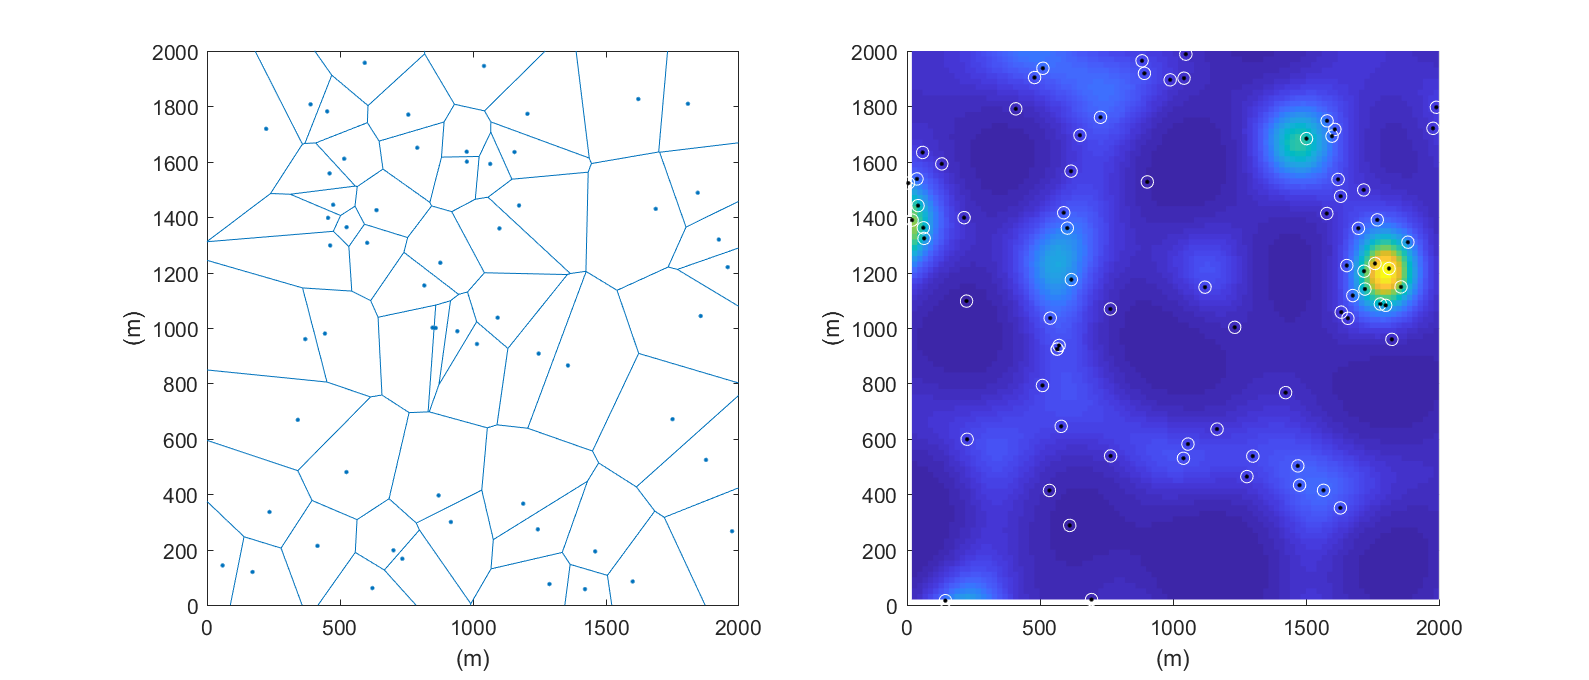
\includegraphics[scale=0.5]{Figures/subplot_BSLocVor_SSLTDPLoc} 

\begin{figure}[h]
\begin{subfigure}{.5\textwidth}
	\centering
	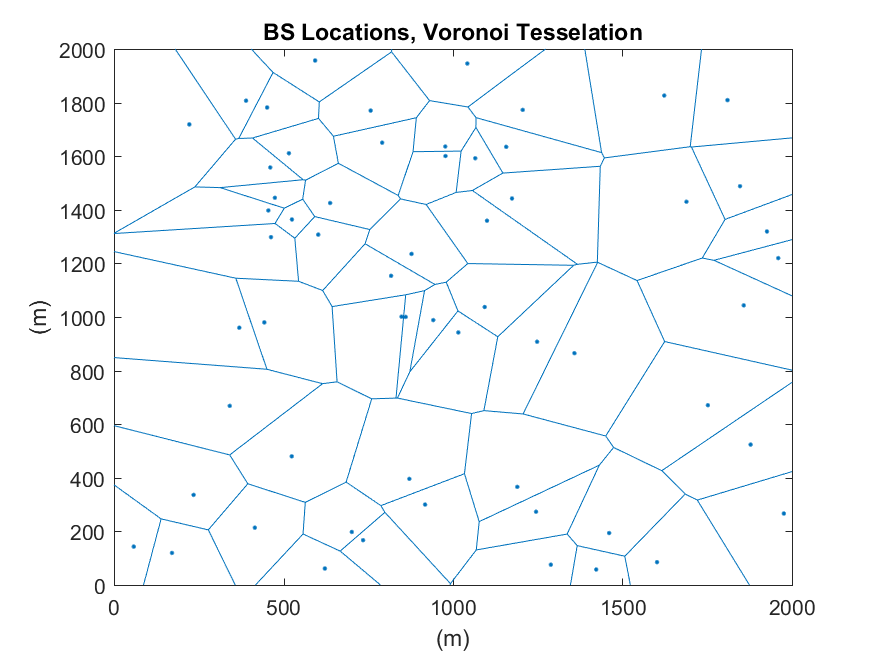
\includegraphics[width=.8\linewidth]{Figures/BSLocationsVoronoi}
	\caption{RP BS Locations in $\mathcal{S}$ with associated Voronoi tesselation}
	\label{fig:BSLocVor}
\end{subfigure}
\begin{subfigure}{.5\textwidth}
	\centering
	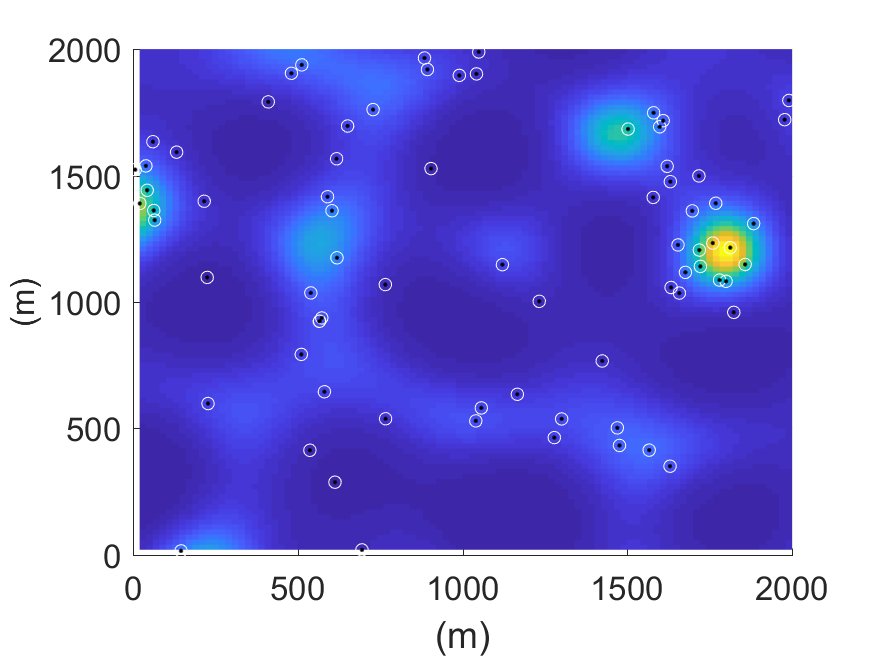
\includegraphics[width=.8\linewidth]{Figures/SSLTnsPPP_demandpointreal}
	\caption{SP SSLT demand density field with one scenario of SP demand points}
	\label{fig:SSLTDPReal}
\end{subfigure}
\caption{Visualization of network area.  (\ref{fig:BSLocVor}) visualizes the resources available to VNB for creating the VWN, and (\ref{fig:SSLTDPReal}) visualizes the demand to be satisfied by the VWN.}
\label{fig:NetworkArea}
\end{figure}

Unless stated otherwise, we use the default parameter vales shown in Table \ref{tab:simval}.  BS locations are determined as a stationary PPP.  Demand point locations are generated independently for each scenario as a non-stationary PPP using $\rho\left(x,\, y\right),\, x \in [0,\, X],\, y \in [0,\, Y]$, as the spatial intensity function, as described in Section \ref{sec:model}.  Fig. \ref{fig:NetworkArea} provides a visualization of the simulation network area.  (\ref{fig:BSLocVor}) shows the BS locations of $\mathcal{S}$ with the associated Voronoi Tesselation showing the coverage areas of the BSs when all are active with respect to the genetic algorithm.  (\ref{fig:SSLTDPReal}) shows the SSLT demand density field with one example scenario of demand points, which acts as a single sample of the demand density field.  To compute $u_{ms}^{\{\omega\}}$, it is assumed that there is perfect propagation between the demand points and BSs.  Unlike as described in Section \ref{sec:model}, $u_{ms}^{\{\omega\}} = 1$ if the distance between demand point $m \in \mathcal{M}$ of scenario $\omega \in \Omega$ and BS $s \in \mathcal{S}$ is less than $b_s$, and 0 otherwise.  To compute the integral of the fitness function (\ref{eq:GACost}), $\rho\left(x,\, y\right)$ is discretized into a grid of congruent pixels, and the demands of all pixels within a Voronoi cell of interest are summed together.

% Mohammad cited CPLEX when he provided the original problem.  Should I, and should I consequently cite MATLAB?
We ran our simulations on an Intel Core i7-4790K 4.00 GHz 4 real core/8 virtual core CPU with 16 GB of DDR3 RAM.  We used CPLEX \cite{Cplex} to solve the DEP optimization problems and we used MATLAB to simulate the genetic algorithm and to generate the demand field and stochastic data (i.e., $\rho\left(x,\, y\right)$ and $u_{ms}^{\{\omega\}}$).  Average values for the performance of the genetic algorithm are provided from 50 independent runs using the identical data set except for the set of initial individuals.  The DEP solutions were solved across multiple values of $\alpha$ as cost, time, and demand satisfaction are directly related to $\alpha$.

\subsection{Results} \label{subsec:results}

\begin{figure}[h]
\begin{subfigure}{.5\textwidth}
	\centering
	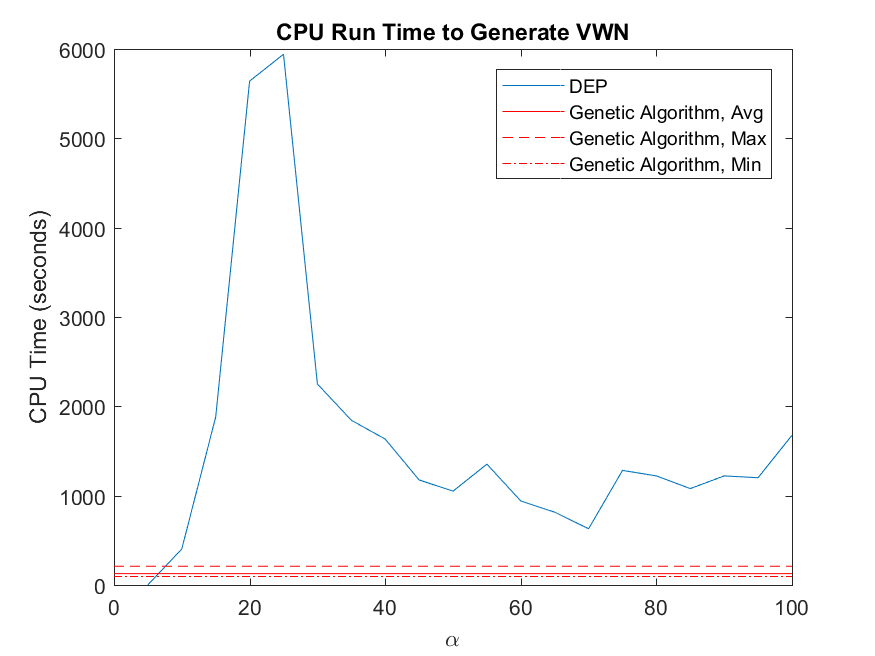
\includegraphics[width=.8\linewidth]{Figures/ComparisonTime}
	\caption{True CPU Time}
	\label{fig:CPUTimeComp}
\end{subfigure}
\begin{subfigure}{.5\textwidth}
	\centering
	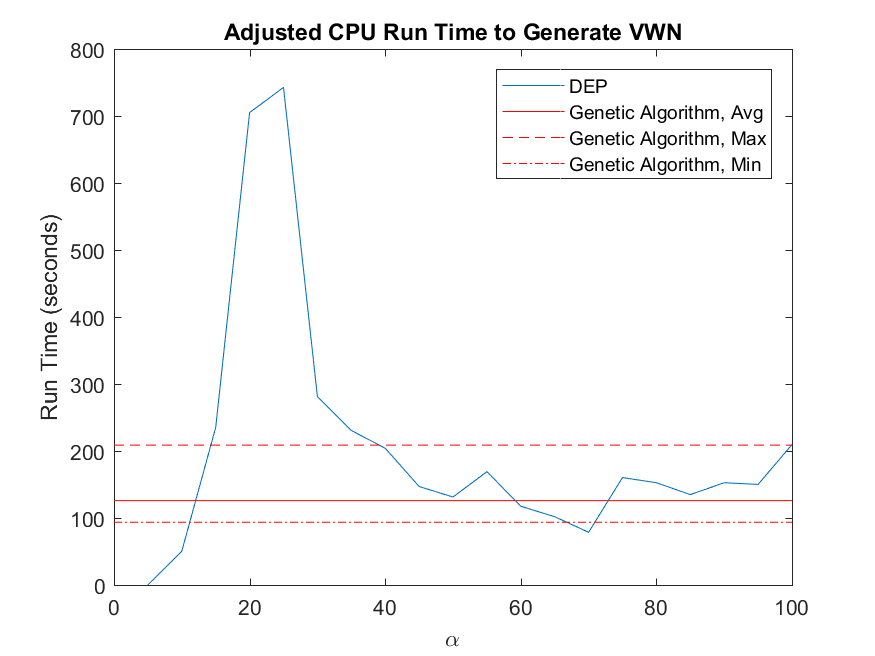
\includegraphics[width=.8\linewidth]{Figures/ComparisonTimeAdjusted}
	\caption{Adjusted (Pseudo-Real) Run Time}
	\label{fig:CPUTimeCompAdj}
\end{subfigure}
\caption{Comparison of Runtimes.  The DEP run time is the solid blue line, while the minimum, average, and maximum genetic algorithm run times are provided as dot-dashed, solid, and dahsed red reference lines, respectively.}
\label{fig:CPUTime}
\end{figure}

In Fig. \ref{fig:CPUTime} is a comparison of the time to run.  (\ref{fig:CPUTimeComp}) shows the absolute overall CPU time taken to converge to a solution in both the DEP and genetic algorithm.  (\ref{fig:CPUTimeCompAdj}) shows an adjusted form of the run time the DEP took to terminate to a single solution.  CPLEX is capable of parallelizing across the 8 CPU cores, allowing for the real run time to take, at minimum, one-eighth of the time.  In comparison, the MATLAB implementation only runs in one core.  With this adjustment providing an improvement to the DEP run time, the genetic algorithm converges in around the same time as the DEP for higher levels of $\alpha$, when a single solution dominates so heavily it simplifies the overall set.  Without the adjustment, the genetic algorithm outperforms the DEP, converging to a solution in 0.125\% the time for $\alpha \geq 30$ and in 0.02\% of the time at $\alpha < 30$.

% Runtime comparison, cost comparison, comment on scalability (increase S, M, or O, and cplex very quickly takes a long time to solve, but the GA is only impacted by S; GA is impacted by I and G_halt and capped in runtime by G, none of which affect DEP, but scale linearly in execution.  GA is further impacted by pixel resolution that DEP is not, but doesn't seem bad considering.
% Should run the GA multiple times for a single value of beta, and see the average results...  That would provide a more solid picture of the consistency of the solutions.
% Should have a figure for rho, a figure of the complete set of demand points as allocated via rho, a figures of selected solutions.
% Should I use a data set that cplex cannot terminate within a reasonable time to solve that the GA easily solves within just a couple minutes?

\noindent {\color{red} \rule{\linewidth}{0.5mm}}

\textit{The following are draft notes for this section:}

In this section, we detail the simulation procedures.  This includes data generation, assumptions, differing models (small and larger scale data sets?), resulting data, how the data is evaluated.  Include the resulting data and potential takeaways from the data.  If solutions are as expected, expand and expound upon it.  If not, then hypothesize why.

Most of this section cannot be worked on until the appropriate data is generated via simulations.  Need optimization and approximation results to compare/contrast against each other.  Approximation data currently seems good, but need optimization results to ensure satisfactory results, especially over a larger data set.

\section{Conclusion} \label{sec:conclusion}

\noindent {\color{red} \rule{\linewidth}{0.5mm}}

\textit{The following are draft notes for this section:}

The conclusion goes here.  Look back on results and reiterate main takeaways.  Include possible avenues for further research and expansion to the model.  Perhaps power control, more nuanced demand-resource allocation (other than basic, simple voronoi), path-loss addition, applying slicing to the genetic algorithm more directly, integrating over the regions in the voronoi GA instead of summing (could be faster; math could be interesting in this or further papers), etc.




% conference papers do not normally have an appendix


% use section* for acknowledgment
%\section*{Acknowledgment}


%The authors would like to thank...





% trigger a \newpage just before the given reference
% number - used to balance the columns on the last page
% adjust value as needed - may need to be readjusted if
% the document is modified later
%\IEEEtriggeratref{8}
% The "triggered" command can be changed if desired:
%\IEEEtriggercmd{\enlargethispage{-5in}}

% references section

% can use a bibliography generated by BibTeX as a .bbl file
% BibTeX documentation can be easily obtained at:
% http://mirror.ctan.org/biblio/bibtex/contrib/doc/
% The IEEEtran BibTeX style support page is at:
% http://www.michaelshell.org/tex/ieeetran/bibtex/
%\bibliographystyle{IEEEtran}
% argument is your BibTeX string definitions and bibliography database(s)
%\bibliography{IEEEabrv,../bib/paper}
%
% <OR> manually copy in the resultant .bbl file
% set second argument of \begin to the number of references
% (used to reserve space for the reference number labels box)
\iffalse
\begin{thebibliography}{2}

\bibitem{IEEEhowto:kopka}
H.~Kopka and P.~W. Daly, \emph{A Guide to \LaTeX}, 3rd~ed.\hskip 1em plus
  0.5em minus 0.4em\relax Harlow, England: Addison-Wesley, 1999.  Sample bib from template.
  
\bibitem{test:teague}
K.~Teague

\end{thebibliography}
\fi

\bibliography{GenAlg_VWN-KTeag}
\bibliographystyle{IEEEtran}


% that's all folks
\end{document}


